\documentclass[a4paper,12pt,oneside]{book}

%-------------------------------Start of the Preable------------------------------------------------
\usepackage[english]{babel}
\usepackage{blindtext}
%packagr for hyperlinks
\usepackage{hyperref}
\hypersetup{
    colorlinks=true,
    linkcolor=blue,
    filecolor=magenta,      
    urlcolor=cyan,
}

\urlstyle{same}
%use of package fancy header
\usepackage{fancyhdr}
\setlength\headheight{26pt}
\fancyhf{}
%\rhead{
\includegraphics[width=1cm]{logo}}
\lhead{\rightmark}
\rhead{
\includegraphics[width=1cm]{logo}}
\fancyfoot[RE, RO]{\thepage}
\fancyfoot[CE, CO]{\href{http://www.e-yantra.org}{www.e-yantra.org}}

\pagestyle{fancy}

%use of package for section title formatting
\usepackage{titlesec}
\titleformat{\chapter}
  {\Large\bfseries} % format
  {}                % label
  {0pt}             % sep
  {\huge}           % before-code
 
%use of package tcolorbox for colorful textbox
\usepackage[most]{tcolorbox}
\tcbset{colback=cyan!5!white,colframe=cyan!75!black,halign title = flush center}

\newtcolorbox{mybox}[1]{colback=cyan!5!white,
colframe=cyan!75!black,fonttitle=\bfseries,
title=\textbf{\Large{#1}}}

%use of package marginnote for notes in margin
\usepackage{marginnote}

%use of packgage watermark for pages
%\usepackage{draftwatermark}
%\SetWatermarkText{
\includegraphics{logo}}
\usepackage[scale=2,opacity=0.1,angle=0]{background}
\backgroundsetup{
contents={
\includegraphics{logo}}
}

%use of newcommand for keywords color
\usepackage{xcolor}
\newcommand{\keyword}[1]{\textcolor{red}{\textbf{#1}}}

%package for inserting pictures
\usepackage{graphicx}

%package for highlighting
\usepackage{color,soul}

%new command for table
\newcommand{\head}[1]{\textnormal{\textbf{#1}}}


%----------------------End of the Preamble---------------------------------------


\begin{document}

%---------------------Title Page------------------------------------------------
\begin{titlepage}
\raggedright
{\Large eYSIP2016\\[1cm]}
{\Huge\scshape Sign Language Interpreter Using Leap Motion Sensor \\[.1in]}
\vfill
\begin{flushright}
{\large Intern: Sanket R Bhimani \\}
{\large Mentor1: Aditya Panwar\\}
{\large Mentor2: Rama Kumar \\}
{\large Duration of Internship: $ 21/05/2016-10/07/2016 $ \\}
\end{flushright}

{\itshape 2016, e-Yantra Publication}
\end{titlepage}
%-------------------------------------------------------------------------------

\chapter[Project Tag]{Sign Language Interpreter\\Using Leap Motion Sensor}
\section*{Abstract}
This project will recognize the gestures performed by hearing impaired or verbally challenged persons and convert it into natural audio.Here, a set of words is taken as input and is then converted into a full grammatically correct sentence using NLTK library.\\
Afterwards, these words in the sentence are mapped with pre-recorded audio file stored in the MP3 module and finally is interpreted through the Galileo Board and is audible via a speaker/headphone.\\
The other part of the project is a robotic hand that tries to imitate the actions of a person's hand when performed over the Leap Motion Sensor. Here Leap sensor's data is mapped with servos' angle through Galileo Board which controls the robotic hand.

\subsection*{Completion status}
Both parts of the project are almost completed. However, in Sign Language Interpreter, making of compact and portable version is remaining. In Robotic Hand making of power supply is left. Currently it is working on LAB DC power supply.
\section{Hardware parts}
\begin{itemize}
  \item Galileo Board \href[page=5]{./datasheet/intel-galileo.pdf}{Datasheet}, \href{http://www.amazon.in/Intel-GALILEO-Microcontroller-Motherboard-GALILEO1-Y/dp/B00K53CQK4?tag=googinhydr18418-21}{Vendor link} 
  \item FN-M16P MP3 module \href[page=5]{./datasheet/FN-M16P_MP3_Module.pdf}{Datasheet}, \href{http://www.electronics123.com/shop/product/mini-embedded-mp3-module-8218}{Vendor link} 
  \item Leap Motion Sensor \href[page=5]{https://developer.leapmotion.com/documentation/}{Documentation}, \href{http://store-world.leapmotion.com/products/leap-motion-controller}{Vendor link} 
  \item GS-5515MG Servo \href[page=5]{./datasheet/GS-5515MG.pdf}{Datasheet},\href{http://www.goodluckbuy.com/goteck-gs-5515mg-15kg-high-troque-analog-metal-gear-servo-for-rc-models.html}{Vendor link}
  \item Any Speaker
  \item 3D Printed parts of Robotic Hand(STL files given in GitHub Repository)
  
\end{itemize}

\section{Software used}
\begin{itemize}
  \item Leap SDK, \href{https://developer.leapmotion.com/v2}{download link},
  \item BitVise SSH Client: version, \href{https://www.bitvise.com/ssh-client-download}{download link}, 
  \item Linux For Galileo \href{https://downloadmirror.intel.com/26028/eng/iot-devkit-prof-dev-image-galileo-20160525.zip}{download link}, {For installation read Galileo Tutorial}
  \item Python Programming Language 2.7 \href{https://www.python.org/download/releases/2.7/}{download link}
  
\end{itemize}

\section{Assembly of hardware}
\textbf{For Sign Language Interpreter,}
\subsection*{Circuit Diagram}
See Figure: 1
\begin{figure}
  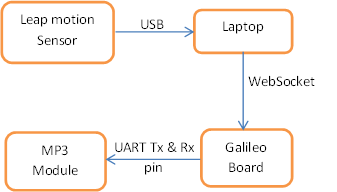
\includegraphics[width=\linewidth]{1.png}
  \caption{Block diagram for SIGN LANGUAGE INTERPRETER hardware system}
\end{figure}
\subsection*{Step 1}
Connect Leap Motion Sensor with PC with USB connection
\subsection*{Step 2}
Connect Galileo Board with PC through WIFI or LAN
\subsection*{Step 3}
Connect MP3 Module With Board.(Just give VCC and GND to module and board's Rx pin to Module's Tx pin and board's Tx pin to module's Rx pin.)(Refer data sheet of MP3 module for pin diagram)\\
\textbf{.1cm}\\
\textbf{For Robotic Hand,}
\subsection*{Circuit Diagram}
See Figure: 2
\begin{figure}
  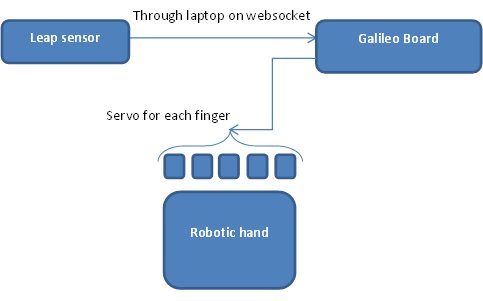
\includegraphics[width=\linewidth]{2.png}
  \caption{Block diagram for Robotic hand system}
\end{figure}
\subsection*{Step 1}
Assemble all 3D printed parts of Hand. Refer \href{http://inmoov.fr/hand-and-forarm/}{this}
\subsection*{Step 2}
Connect Leap Motion Sensor with PC with USB
\subsection*{Step 3}
Connect PC with Galileo using LAN or WIFI
\subsection*{Step 4}
Connect PWM pin of servo to Board's PWM output pin(For Connection refer Galileo\_board\_tutorial)\\
Provide 5V DC power supply to each servo. Make sure, 700mA current is provided to each servo.

\section{Software and Code}
\href{https://github.com/eYSIP-2016/eYSIP-2016-Sign-Language-Interpreter-Leap-Motion-Sensor-}{Github link} for the repository of code\\
\vspace{.3cm}\\
\textbf{For Sign Language Interpreter:}\\
\vspace{.3cm}\\
There are two programs, one is for PC/Laptop and another is for Galileo Board. One script will be running on board to catch massages sent through PC. This script will also handle all the tasks related to the interfacing of MP3 module to play any audio file via UART communication. And One script will be running on PC to recognizing Gestures and interpret them in words. The second script will be running on PC/Laptop to recognize gestures and interpret them as words.
The tasks related to making natural sentences (grammatically correct) from words and making grammar are also carried out by this particular script. This thing will be done through NLTK library.\\
Task Achieved with each program:\\
\vspace{1cm}\\
\textbf{\Large{on\_laptop.py}}\\
\begin{itemize}
\item \textbf{Recognizing Gesture:}\\
For gesture recognition two parameters each figures position and direction of all three axis are counted. And also relate them with palm center to make independent of palm position from sensor. Now program takes 300 frame to record record the gesture and then all data is stored in JSON file as a permanent copy. Now when program is restarted all gesture will be loaded from that JSON file. For recognizing gesture again it will take 300 frame and compare with saved frame. Then in whichever gesture higher frames matched is become  the result. For making this system faster, all data is converted into matrix and all processes are done through numpy. 
\item \textbf{Making of sentence:}\\
After Recognizing single words, a set of words is generated. Then this set become sentence here. For example, if set is ['What', 'name', 'you'], then here some words are added to make proper sentence and it also corrects the places of word. So, here the output for above set will be ['what', 'is', 'you', 'name']. Then grammar will be corrected in next module.
\item \textbf{Correcting Grammar}\\
Here Grammar of sentence is corrected.. For that, I have used online API of Ginger grammar. So this will make ['what', 'is', 'you', 'name'] to ['what', 'is', 'your', 'name'].
\item \textbf{Sending sentence to board}\\
Then this sentence is sent to board through websocket here this code become client and board become server.
\end{itemize}
\textbf{\Large{on\_board.py}}
\begin{itemize}
\item Receiving sentence\\
Receive the sentence through websocket.
\item Differentiate each word from sentence and map with file number.
\item Generate hex code for MP3 module\\
MP3 module needs hex code to perform specific task. So here proper hex code is generated. hex code also includes check bits counting.
\item Sending hex code to MP3 module\\
then this generated hex code is sent to mp3 module through UART.
\end{itemize}
\vspace{.3cm}
\textbf{For Robotic hand:}\\
\vspace{.3cm}\\
\textbf{Laptop side program}\\
Here Leap data is mapped to servo angle. Here, two parameters are used, one is \textbf{tip position's y axis} and \textbf{palm center's y axis}. and \textbf{tip position's y axis} is relate to palm center. So, it become independent from hand position. Then Send data of all five angle of each finger to board through websocket\\
\textbf{Board side program}\\
It just receive angle and data and generate PWM signal according to that.
\section{Use and Demo}
\textbf{For Sign Language Interpreter}\\
See Figure: 3\\
\begin{figure}
  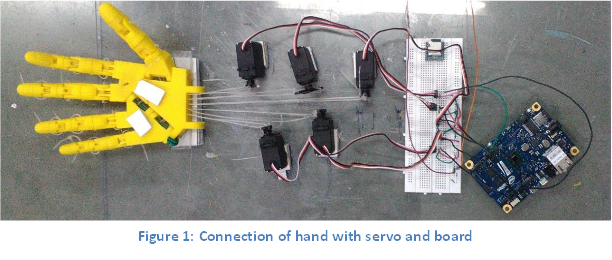
\includegraphics[width=\linewidth]{3.png}
  \caption{Connection between MP3 module and Galileo}
\end{figure}
\textbf{step 1:}\\
Connect board,mp3 module.....as shown in Figure: 3\\
\textbf{step 2:}\\
Connect board with SSH to pc\\
\textbf{step 3:}\\
Enter IP of board in on\_laptop.py\\
\textbf{step 4:}\\
run on\_board.py on Galileo board.\\
\textbf{step 5:}\\
run on\_laptop.py on laptop\\


For better recognition, sit on chair and put leap on table and before performing any new gesture show whole palm first.\\
\vspace{1cm}\\
\textbf{For Robotic Hand}\\
\href{https://youtu.be/T554uLQ0PaI}{Youtube Link} of demonstration video 

See Figure: 4\\

\begin{figure}
  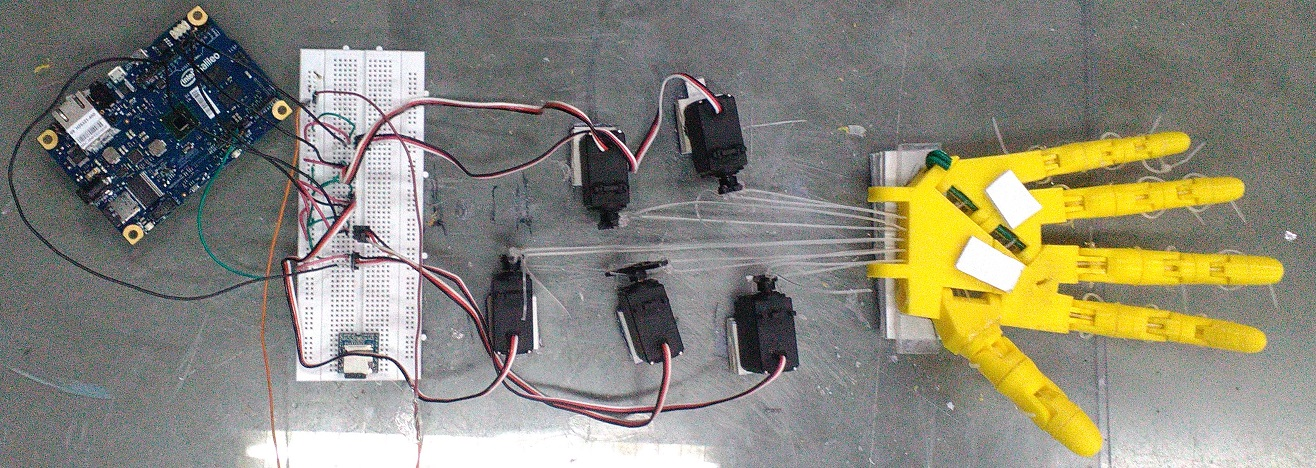
\includegraphics[width=\linewidth]{4.jpg}
  \caption{Connection for robotic hand}
\end{figure}
\textbf{step 1:}\\
Make all connection with board, servos, leap and pc\\
\textbf{step 2:}\\
connect board with SSH to pc\\
\textbf{step 3:}\\
Enter IP of board in follow\_hand\_client.py\\
\textbf{step 4:}\\
run follow\_hand\_server.py on Galileo board.\\
\textbf{step 5:}\\
run follow\_hand\_client.py on laptop\\

Now perform pose on leap at least 15CM above the sensor.


\section{Future Work}
\textbf{For Sign language Recognizing system,}\\
\begin{itemize}
\item Make whole system portable and compact like a tablet and make it more accurate.
\item Word dictionary can be reach with all necessary words.
\end{itemize}

\textbf{For robotic hand,}\\
Make more joints accessible.

\section{Bug report and Challenges}
\textbf{Bug report:}\\
The gesture of people other than the trainer who trained the system does not produce efficient output.\\
\textbf{Challenges:}\\
Initially, Reorganization was not accurate. Error rate was almost 50\%. that was some LeapTrainer.js library. So I've decided to make my own thing. So I made algorithm, Now challenge is to make it faster. Because it was too slow. It take 18-21 seconds to recognize single word. So, I converted all data in form of matrix and so, I could use numpy library. Numpy library complete tasks at most efficient and faster way. So my reorganization become more faster, Now it takes only 0.3 second to recognize word.\\
In robotic hand there was a problem of power supply because I need 5V with 5A power supply. It was quit hard to build such supply. So, currently I am using LAB DC power supply.

\begin{thebibliography}{li}
\bibitem{wavelan97}
Robotic hand STL files,
{\em http://inmoov.fr/hand-and-forarm/.}
\bibitem{wavelan97}
{\em https://github.com/intel-iot-devkit/mraa/}

\bibitem{wavelan97} 
{\em www.developer.leapmotion.com/documentation/python/index.html}
\bibitem{wavelan97} 
{\em www.nltk.org}
\bibitem{wavelan97} 
{\em www.youtube.com/watch?v=FLZvOKSCkxY}
\bibitem{wavelan97} 
{\em www.gingersoftware.com/grammarcheck}
\bibitem{wavelan97} 
{\em www.github.com/zoncoen/python-ginger}
\bibitem{wavelan97} 
{\em www.blog.livedoor.jp/xaicron/archives/54466736.html}
 \bibitem{wavelan97} 
{\em www.youtube.com/watch?v=gN3CGhFPF1s}
 \bibitem{wavelan97} 
{\em www.downloadmirror.intel.com/26028/eng/iot-devkit-prof-dev-image-
galileo-20160525.zip}
 \bibitem{wavelan97} 
{\em www.software.intel.com/en-us/iot/hardware/galileo/downloads}
\bibitem{wavelan97} 
{\em www.downloadmirror.intel.com/25384/eng/w galileo 2015.0.010.exe}
\bibitem{wavelan97} 
{\em www.youtube.com/watch?v=yrRMomesBKM}
\bibitem{wavelan97} 
{\em www.github.com/intel-iot-devkit/mraa}
\end{thebibliography}


\end{document}

